\documentclass[10pt]{jhwhw}
\author{Ian Malerich}
\title{Math S 373: Final Assignment}
\usepackage{amssymb, amsfonts, amsmath, mathtools, graphicx, breqn, soul}
\usepackage{minted, subfig, float, scrextend, setspace, amsthm}
\usemintedstyle{friendly}

\begin{document}
\raggedright

%% Problem 1
\problem{} (60 points)

	Consider the initial value problem (IVP) for the ordinary differential
	equation (ODE):
	\begin{align*}
		y'(t) = \frac{dy}{dt} &= \sin(y(t)), t\in [0, 1] \\
		y(0) &= 1
	\end{align*}
	Let's partition the domain [0, 1] into $n$ sub-intervals equally with mesh
	size $h = 1/n$, i.e., $0=t_0 < t_1 < \cdots < t_{n-1} < t_n = 1$ with 
	$t_k = k/n$ for $k = 0, 1, \ldots, n$. We will find approximation of the solution
	$y(t)$ at the grid points $\{t_0, t_1, \ldots, t_n\}$ as $y_k \approx y(t_k)$ for
	$k = 0,1,\ldots,n$. It is obvious that $y_0 = 1$ by the initial condition. \\
	Implement the following methods with Matlab (using $n=20,40$) and plot the results.

	\begin{enumerate}
		\item
			At each point $t_k$, approximate the derivative $y'(t_k)$ with forward
			difference to get
			$$
				y_{k+1} = y_k + h\sin(y_k)
			$$
		\item
			At each point $t_k$, approximate the derivative $y'(t_k)$ with backward
			difference to get 
			$$
				y_{k+1} = y_k + h\sin(y_{k+1})
			$$
			To obtain update $y_{k+1}$, use Fixed point iteration to solve the nonlinear
			equation for $y_{k+1}$ (using $y_k + h\sin (y_k)$ as initial guess
			in the Matlab routine for fixed point iteration).
		\item
			Take integral of the ODE from $t_k$ to $t_{k+1}$ to get
			$$
				y_{k+1} = y_k + \int_{t_k}^{t_{k+1}} \sin(y(t))dt,
			$$
			and use Trapezoidal rule to approximate the above integral to get
			$$
				y_{k+1} = y_k + h\frac{\sin(y_k) + \sin(y_{k+1})}{2}.
			$$
			To obtain update $y_{k+1}$, use Fixed point iteration to solve the nonlinear
			equation for $y_{k+1}$ (using $y_k + h\sin (y_k)$ as initial guess
			in the Matlab routine for fixed point iteration).
	\end{enumerate}

\clearpage
\solution

	\part

	\inputminted{octave}{p1a.m}
	Below we can see the results of plotting the results of $p1a(20)$ and $p1a(40)$.
	Where left (blue) is $n=20$ and the right (red) is $n=40$. \\
	\begin{centering}
		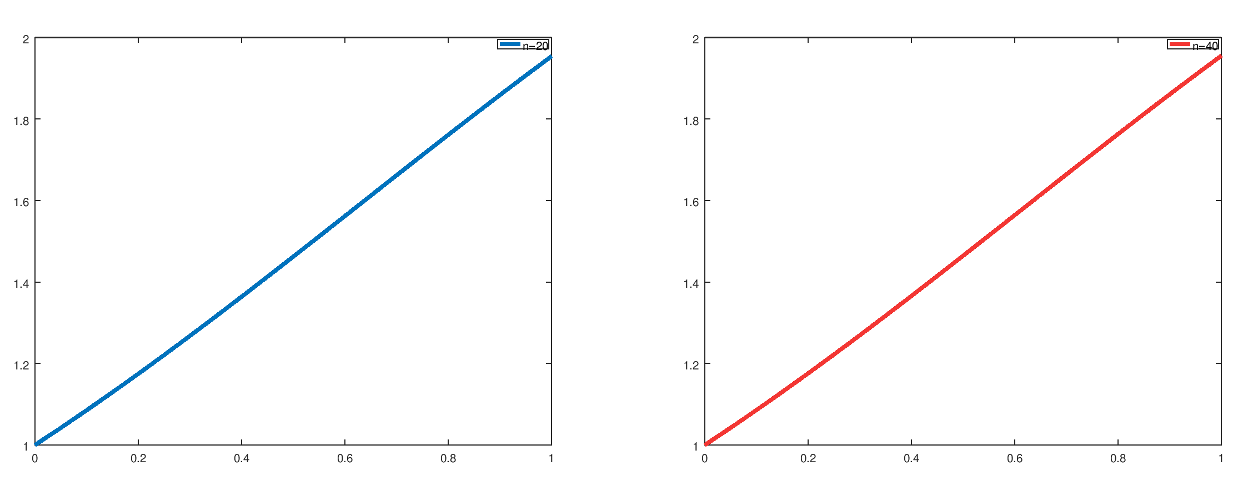
\includegraphics[scale=0.85]{p1a.png}
	\end{centering}

	\clearpage
	\part
	\inputminted{octave}{p1b.m}
	Again we get very similar looking results by running this method with step sizes
	$n=20,40$. Below you can see a plot of the results of calling the above Matlab code.
	The left (blue) is for $n=20$ and the right (purple) for $n=40$.
	\begin{centering}
		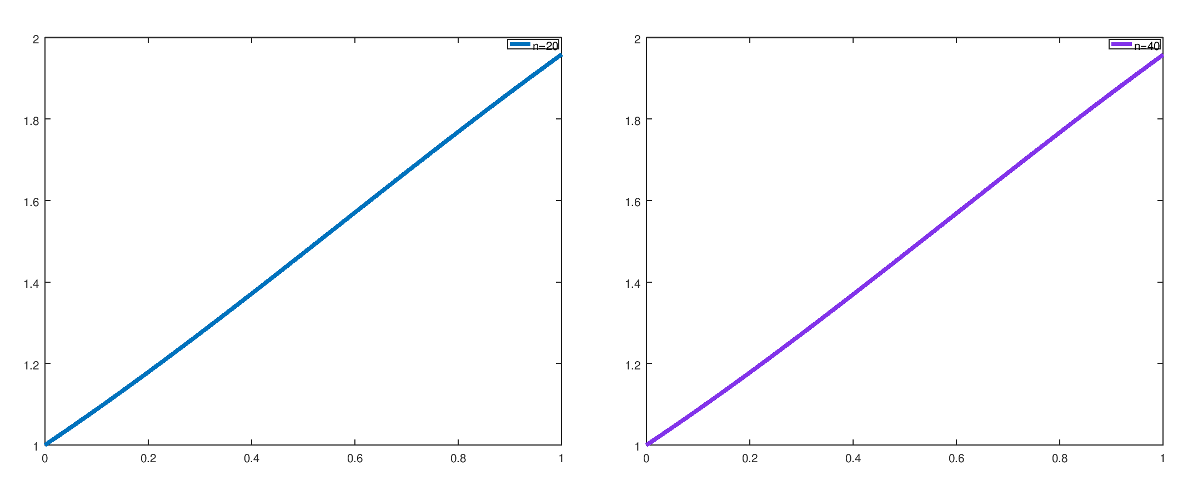
\includegraphics[scale=0.85]{p1b.png}
	\end{centering}

	\clearpage
	\part
	\inputminted{octave}{p1c.m}
	The code for this method is very similar to part b, only requiring an update to the 
	function which computes the next value (though it takes the same parameters).
	Below you can see a plot af the results of calling the above Matlab code.
	The left (blue) is for $n=20$ and the right (green) for $n=40$.
	\begin{centering}
		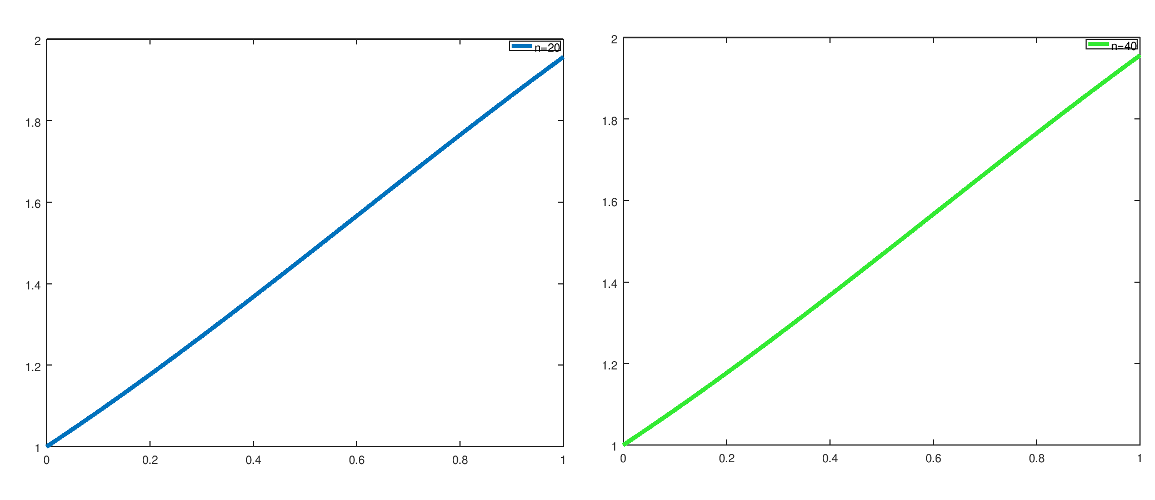
\includegraphics[scale=0.85]{p1c.png}
	\end{centering}

%% Problem 2
\problem{} (40 points)

	Consider the Boundary value problem for the Poisson equation:
	\begin{align*}
		-u''(x) &= f(x), x\in [0,1] \\
		u(0) = \alpha&, u(1) = \beta.
	\end{align*}
	Let's partition the domain $[0,1]$ into $n$ subintervals equally with mesh size
	$h=1/n$, i.e. $0=x_0 < x_1 < \cdots < x_{n-1} < x_n = 1$, with $x_k = k/n$ for
	$k = 0, 1, \ldots, n$. We will find an approximation of the solution $u(x)$ at the grid
	points $\{x_0, x_1, \ldots, x_n\}$ as $u_k \approx u(x_k)$ for $k=0,1,\ldots,n$.
	It is obvious that $u_0 = \alpha, u_n = \Beta$ by the Boundary condition. \\
	At each point $x_k$ for $k=1,2,\ldots,n-1$, approximate the second derivative $u''(x_k)$
	using three-point central difference
	$$
		u''(x_k) \approx \frac{u(x_{k+1}) - 2u(x_k) + u(x_{k-1})}{h^2}
	$$
	With the above approximation to set up a linear system to determine
	$\{u_1, u_2, \ldots, u_{n-1}\}$, i.e.,
	$$
		A\mathbf{u} = \mathbf{b}
	$$
	with 
	$$
	A = \begin{bmatrix}
		2 & -1 & \cdots & \cdots & 0 \\
		-1 & 2 & -1 & \cdots & 0 \\
		\vdots & \ddots & \ddots & \ddots & \\
		0 & \cdots & -1 & 2 & -1 \\
		0 & \cdots & \cdots & -1 & 2 \\
	\end{bmatrix},
	u = \begin{bmatrix}
		u_1 \\
		u_2 \\
		\vdots \\
		u_{n-2} \\
		u_{n-1} \\
	\end{bmatrix},
	b = \begin{bmatrix}
		f_1 + u_0/h^2 \\
		f_2 \\
		\vdots \\
		f_{n-2} \\
		f_{n-1} + u_n/h^2
	\end{bmatrix}
	$$
	Implement the above method with Matlab and plot the results. 
	Choose $f(x) = 4\sin(2x), \alpha = 0, \beta = \sin(2), n=20,40$.
	\begin{enumerate}
		\item Find the maximum and minimum eigenvalues (in magnitude) of A.
		\item solve the linear system by Gaussian Elimination with Backward substitution.
	\end{enumerate}

\solution

\end{document}
